% Exact symmetry-stratified search for fast matrix multiplication over F_2
% Author: Nadim F. Zaru

\documentclass[11pt]{article}
\usepackage[utf8]{inputenc}
\usepackage[margin=1in]{geometry}
\usepackage{amsmath,amsthm,amssymb}
\usepackage{graphicx}
\usepackage{hyperref}
\usepackage{booktabs}
\usepackage{algorithm}
\usepackage{algorithmic}
\usepackage{xcolor}

\newtheorem{theorem}{Theorem}
\newtheorem{lemma}{Lemma}
\newtheorem{corollary}{Corollary}
\newtheorem{definition}{Definition}
\newtheorem{proposition}{Proposition}
\newtheorem{remark}{Remark}

\newcommand{\FF}{\mathbb{F}_2}
\newcommand{\tw}[3]{\langle #1,#2,#3\rangle}
\newcommand{\GL}{\mathrm{GL}}

\emergencystretch=3em
\hbadness=10000

\title{%
  \textbf{Exact Symmetry-Stratified Search for Fast Matrix \\
  Multiplication over $\FF$: A Second Inequivalent \\
  Rank-47 Scheme for $4\times4$, Rigidity Theorems, \\
  and Large Same-Rank Families at $5\times5$ and $6\times6$}
}

\author{
  Nadim F. Zaru \\
  \textit{Independent Researcher} \\
  \texttt{nadimzaru@gmail.com}
}

\date{September 9, 2026}

\begin{document}

\maketitle

\begin{abstract}
We report an exact, symmetry-stratified computational search for bilinear matrix-multiplication schemes
over $\FF$, carried out on one consumer laptop. Every scheme reported here was accepted only after an
exact check of all $n^6$ Brent equations, and every negative result is a solver refutation, never a
budget exhaustion. Five contributions. (1) The rank-47 $\tw444$ factorization published by AlphaTensor is
exactly invariant under a group $\Gamma$ of order 12 --- an $S_3$ of permutation sandwiches together with a
transpose-swap involution --- with orbit sizes $12,6,6,6,6,3,3,3,1,1$; we did not find this structure
reported in the sources we consulted. (2) Searching from scratch for a $\Gamma$-invariant scheme with that
orbit type produced a \emph{second} host-verified rank-47 scheme for $\tw444$ over $\FF$ that shares no
term with AlphaTensor's, has a different $\GL(4,2)^3$-invariant factor-rank signature, and is therefore
inequivalent to it under every change of basis and slot symmetry. (3) Both rank-47 schemes are locally
rigid: exhaustive orbit-level rewrites --- 28{,}835 decided SAT instances, with no budget exhaustion remaining --- refute
every $\Gamma$-invariant rank-46 scheme that keeps 8 or more of the 10 orbits of either scheme, and every
other $\Gamma$-invariant rank-47 scheme within the searched rewrite radius. Both are also
\emph{flip-isolated}: no two terms share a factor on any axis, so no flip-graph move can act on them. (4) A
fixed-point restriction lemma for involution-symmetric schemes: the Brent equations at involution-fixed
coordinates close on the involution-fixed terms alone, and for block-preserving involutions those terms
restrict to a scheme for a smaller matrix format. The lemma refutes symmetry classes at essentially zero
cost --- 892 of 11{,}767 census instances outright, and 21{,}647 of the first 23{,}072 orbit-type
multisets of a rank-46 census --- and re-derives $\mathrm{rank}_{\FF}\tw222 = 7$ by SAT. (5) At $5\times5$
and $6\times6$ the published rank-93 and rank-153 schemes sit in large families of same-rank schemes
connected by exact two-orbit rewrites: 307 and 79 distinct host-verified members respectively, where one
was previously known, with at least 272 and 47 pairwise-inequivalent classes. No rank-46, rank-92 or
rank-152 scheme was found, and none exists within any of the exhaustively searched neighbourhoods.

\textbf{Keywords:} bilinear complexity, matrix multiplication, Brent equations, finite fields, SAT
solving, symmetry breaking, flip graphs, AlphaTensor
\end{abstract}

\section{Introduction}

The number of scalar multiplications needed to multiply two $n\times n$ matrices is the bilinear rank of
the matrix-multiplication tensor $\tw nnn$. Strassen's 1969 scheme~\cite{Strassen1969} showed
$\mathrm{rank}\tw222 \leq 7$, and Winograd~\cite{Winograd1971} proved 7 optimal. Beyond $2\times2$ the
exact ranks are unknown, and progress comes from explicit constructions. Two recent lines produced most
of the current small-format records: the reinforcement-learning search of AlphaTensor~\cite{Fawzi2022},
which found a rank-47 scheme for $\tw444$ over $\FF$ (the first improvement on
Strassen$^{\otimes2}$'s 49 for that format over any field), and the flip-graph
method~\cite{Kauers2022,Arai2024,Moosbauer2025}, a local-search dynamic on the space of
correct schemes that produced the current $5\times5$ rank-93 and $6\times6$ rank-153 schemes.

This paper reports a campaign that set out to beat 47 at $4\times4$ over $\FF$ and did not. It failed in a
specific and informative way, and the machinery built to fail informatively produced results of
independent interest: exact structural theorems about the known records, a second inequivalent rank-47
scheme, and hundreds of new verified schemes at $5\times5$ and $6\times6$.

The organising idea throughout is \emph{symmetry stratification}. A scheme of rank $r$ that is invariant
under a group $G$ acting on the tensor's coordinates decomposes into $G$-orbits of terms, and is
determined by one representative per orbit. Fixing $G$ and an orbit-size multiset summing to $r$ turns
the search for a rank-$r$ scheme into a SAT instance with roughly $|G|$ times fewer free variables than
the unrestricted problem. Refutations then become theorems of the form ``no rank-$r$ scheme with this
symmetry and this orbit type exists,'' and satisfying assignments become schemes, which we verify
exactly before reporting.

\subsection{Contributions}

\begin{itemize}
\item \textbf{The symmetry group of AlphaTensor's 47} (Section~\ref{sec:gamma}): order 12, $S_3\times
\langle\tau\rangle$, ten orbits of sizes $12,6,6,6,6,3,3,3,1,1$. Determined by exhaustive search of
$\GL(4,2)^3$ sandwiches with rank-one pruning, and re-verified term by term.
\item \textbf{A second inequivalent rank-47 scheme for $\tw444$ over $\FF$}
(Section~\ref{sec:second47}), found from scratch under the same symmetry and orbit type: zero terms in
common with AlphaTensor's, a different $\GL$-invariant factor-rank signature, and not the image of
AlphaTensor's under any of the 82{,}944 permutation-and-slot symmetries. Both schemes are printed term
by term in the supplement.
\item \textbf{Rigidity and isolation theorems} (Sections~\ref{sec:rigidity}, \ref{sec:obstructions}) for
both rank-47 schemes and for the $5\times5$ and $6\times6$ records, each an exhaustive UNSAT sweep with
no budget exhaustions, together with three basis-independent obstructions: flip isolation, non-liftability
to $\mathbb{Z}/4$, and a Kronecker-rank obstruction that rules out any ``Strassen$^{\otimes2}$ plus a
correction'' ansatz for the 47 in every basis.
\item \textbf{A fixed-point restriction lemma} (Section~\ref{sec:fixedpoint}) with a corollary that
bounds the number of involution-fixed terms below by the bilinear rank of a smaller format. As a filter it
is essentially free and refutes a large fraction of symmetry classes outright; as a by-product it
re-derives $\mathrm{rank}_{\FF}\tw222 = 7$ by SAT.
\item \textbf{Large same-rank families at $5\times5$ and $6\times6$} (Section~\ref{sec:families}): 307
and 79 distinct host-verified $C_3$-invariant schemes at the record ranks, produced by exact two-orbit
rewrites, none of which descends by any tested method.
\end{itemize}

\subsection{What this work does not claim}

No published record is improved. The negative results are exact but local: they concern specific symmetry
groups and specific rewrite radii, and say nothing about schemes outside them. Section~\ref{sec:scope}
states the scope of each class of result precisely.

\subsection{Computational infrastructure}

All computations ran on one laptop: an NVIDIA GeForce RTX 5070 Laptop GPU (8\,GB) for the flip-graph
walkers, and 12 physical CPU cores for the SAT work, using CaDiCaL 1.9.5~\cite{cadical} through
PySAT~\cite{pysat}. The per-instance logs aggregated for this paper account for 352.9 solver-hours over
311{,}872 instance records, plus approximately 6 GPU-hours of logged walks.

\section{Background and Preliminaries}

\subsection{Bilinear schemes and the Brent equations}

\begin{definition}[Scheme]
A \emph{scheme} of rank $r$ for $\tw nnn$ over $\FF$ is a list of $r$ triples $(a_t,b_t,c_t)$ of
$n\times n$ matrices over $\FF$ such that, for all index quadruples,
\begin{equation}
\sum_{t=1}^{r} a_t[i,j]\, b_t[j',k]\, c_t[k',i'] \;=\; [j=j']\,[k=k']\,[i=i'] \pmod 2 .
\label{eq:brent}
\end{equation}
\end{definition}

These are the Brent equations~\cite{Brent1970}; there are $n^6$ of them ($4096$ for $n=4$). The minimum
$r$ over all schemes is the bilinear rank of the tensor. We store each factor as an $n^2$-bit mask, bit
$ni+j$ holding entry $(i,j)$, and we call a scheme \emph{host-verified} when a direct evaluation of
all $n^6$ equations accepts it. Every scheme reported in this paper is host-verified; the verifier was
itself validated by rejecting single-bit corruptions of accepted schemes and by accepting the trivial
rank-$n^3$ scheme.

\subsection{Symmetries}

Two kinds of symmetry act on schemes. \emph{Sandwiching} by a triple $(X,Y,Z)\in\GL(n,2)^3$ sends
$(a,b,c)\mapsto (XaY^{-1},\,YbZ^{-1},\,ZcX^{-1})$ and preserves the target tensor; so does the
\emph{cyclic slot rotation} $\mathrm{cyc}:(a,b,c)\mapsto(b,c,a)$ and the \emph{transpose swap}
$\tau:(a,b,c)\mapsto(b^{\mathsf T},a^{\mathsf T},c^{\mathsf T})$. The full automorphism group is
$\GL(n,2)^3\rtimes S_3$. Restricting the sandwiches to permutation matrices gives an ambient group
$\Omega$ of order $82{,}944$ at $n=4$, which we use as the reference group for equivalence tests.

\begin{definition}[Factor-rank signature]
The \emph{factor-rank signature} of a scheme is, for each of the three axes, the histogram of the $\FF$
matrix ranks of its factors on that axis.
\end{definition}

Since sandwiching by invertible matrices preserves matrix rank, the signature is a
$\GL(n,2)^3$-invariant, and the multiset of the three per-axis histograms is invariant under the whole
automorphism group. Two schemes with different signature multisets are therefore inequivalent, in every
basis and under every slot symmetry. This is the invariant we use for all inequivalence claims.

\begin{definition}[Flip isolation]
A scheme is \emph{flip-isolated} when no two of its terms share a factor on any axis.
\end{definition}

The flip-graph method~\cite{Kauers2022} moves between schemes by \emph{flips}, which require two terms
sharing a factor, and reduces rank by \emph{reductions}, which require two terms sharing two factors. A
flip-isolated scheme therefore admits no flip and no reduction, and since sharing is preserved by
sandwiching, so does every scheme equivalent to it.

\subsection{Known records and bounds}

\begin{center}
\begin{tabular}{lccl}
\toprule
Format & Best known rank & Field & Source \\
\midrule
$2\times2$ & 7 & any & Strassen 1969~\cite{Strassen1969}; optimal~\cite{Winograd1971} \\
$3\times3$ & 23 & any & Laderman 1976~\cite{Laderman1976} \\
$4\times4$ & 49 & any & Strassen$^{\otimes2}$ \\
$4\times4$ & \textbf{47} & $\FF$ & AlphaTensor~\cite{Fawzi2022} \\
$5\times5$ & 93 & $\mathbb{Z}$ & Moosbauer--Poole 2025~\cite{Moosbauer2025} \\
$6\times6$ & 153 & $\mathbb{Z}$ & Moosbauer--Poole 2025~\cite{Moosbauer2025} \\
\bottomrule
\end{tabular}
\end{center}

The 47 is an $\FF$-only result; over the rationals the $4\times4$ record remains 49. We imported the
AlphaTensor factorization from the published repository and the $5\times5$ and $6\times6$ schemes from
the Lille FMM database~\cite{fmmdb}, reduced them mod 2, searched all six slot permutations and eight
transpose combinations for the index layout, and re-verified each with our own checker before use. All
three verify under the identity layout.

\subsection{Rules of evidence}
\label{sec:evidence}

Every statement below carries one of four tags. \textbf{[verified]}: an exact host certificate of a
concrete scheme. \textbf{[exact]}: a solver UNSAT result or an exhaustive computation with no budget
exhaustion. \textbf{[measured]}: an observed rate, count or floor. \textbf{[open]}: unknown. Instances
that exhausted a conflict budget are reported as undecided and never counted as refutations. Every
satisfying assignment is decoded and host-verified before it is called a scheme.

\section{Methodology}
\label{sec:method}

\subsection{Orbit-level encoding}

Fix a group $G$ acting on the $3n^2$ bit positions of a term, a target rank $r$, and a
\emph{slot list}: a multiset of subgroups $H_1,\dots,H_m$ of $G$ with $\sum_i [G:H_i] = r$. A
$G$-invariant scheme of that orbit type is determined by one representative term per slot, constrained to
have stabilizer containing $H_i$. Encoding the Brent equations~(\ref{eq:brent}) over these
representatives, with the images generated as fixed Boolean combinations of the representatives' bits,
gives a SAT instance in $3n^2 m$ free variables instead of $3n^2 r$.

Two exact reductions shrink these instances by roughly a factor of sixteen at $n=4$ with provably
identical verdicts:

\begin{description}
\item[E1, orbit equations.] Because an encoded scheme is a sum of complete $G$-orbits, the Brent
equations at coordinates in the same $G$-orbit are literally the same constraint. Emitting one equation
per orbit of coordinates is exact, not a relaxation.
\item[E2, gate sharing.] The degree-3 monomials $a[i,j]b[j,k]c[k,i]$ recur across equations; introducing
one Tseitin variable per distinct monomial and reusing it removes the duplication.
\end{description}

Both were validated by cross-checking every verdict against the unreduced encoding on an exhaustive
$n=2$ census (44 of 44 instances agreeing) and by recovering the 47 from its own orbit type.

\subsection{Orbit-level rewriting}

To test a known scheme $S$ for local rigidity we delete a set $D$ of its $G$-orbits, keep the rest folded
into the right-hand side as a residual, and ask for a refill: new $G$-orbits whose sizes sum to
$|D|_{\mathrm{terms}}-1$ (a \emph{reduce} instance, target rank $r-1$) or to
$|D|_{\mathrm{terms}}$ (a \emph{same-rank} instance). Stabilizer subgroups are deduplicated up to
conjugacy in $G$, which is exact because conjugate stabilizers give isomorphic instances, and equal-size
refill orbits are unordered. Folding the kept orbits into the residual reduced instances from about
574{,}000 to about 4{,}400 variables.

For same-rank instances the input scheme must be blocked, or the solver simply returns it. We block at
the \emph{set} level --- a clause asserting that the decoded term set differs from the blocked one --- not
at the assignment level, so that relabelings of the same scheme are excluded rather than re-found. An
early version of the campaign blocked at the assignment level and consequently over-counted distinct
solutions; the corrected counts are the ones reported here.

\subsection{The fixed-point filter}
\label{sec:fixedpoint}

Section~\ref{sec:lemma} states the lemma. Operationally it gives two tests that run before any full
solve:

\begin{enumerate}
\item A \emph{count bound}: for each involution $g\in G$ with fixed coordinates, the number of $g$-fixed
terms must be at least the rank of the smaller format the fixed part restricts to. The slot list
determines the fixed count exactly, so this test costs nothing.
\item A \emph{projected subsystem}: the Brent equations at $g$-fixed coordinates, in the $g$-fixed terms
only, form a closed SAT subsystem. It is a projection of the full instance, so UNSAT on the subsystem
implies UNSAT on the instance. It is small and usually decides in milliseconds; instances that exhaust
its budget are passed on to the full solve.
\end{enumerate}

\subsection{General-linear symmetry}

Every symmetry used in the literature we consulted at $4\times4$, and every symmetry used above, is built
from permutation matrices. The automorphism group is larger: $\GL(4,2)$ contains elements of order 3, 5,
7 and 15 that no permutation matrix imitates. We built an encoder for arbitrary sandwich subgroups of
$\GL(4,2)^3$, in which a slot's representative is parametrised by a basis of its stabilizer's fixed space
and the orbit images are XOR combinations of those parameters. It was validated by recovering the 47
under the $S_3$ part of its group and by re-finding a rank-7 $\tw222$ scheme from scratch under an
order-3 element of Strassen's stabilizer.

\subsection{Flip-graph walkers}

For comparison and for seed generation we implemented flip-graph walkers on the GPU: 32{,}768 independent
walks per launch with on-device flips, reductions and plus transitions, and host re-verification of every
claimed improvement. Peak throughput was $3.9\times10^{8}$ flip steps per second. Variants include a
population walker with elite migration and evolved per-block policies, and a $\tau$-quotient walker that
moves entirely within the transpose-symmetric subspace using a closed symmetric move set that includes
two $3\to2$ reductions the plain flip graph cannot express.

\section{Results I: the symmetry of AlphaTensor's rank-47 scheme}
\label{sec:gamma}

\textbf{[verified]} A direct check of all 47 terms shows the scheme is invariant under
$\tau:(a,b,c)\mapsto(b^{\mathsf T},a^{\mathsf T},c^{\mathsf T})$, with 11 fixed terms and 18 swapped
pairs. An exhaustive search of $\GL(4,2)^3$ sandwiches, pruned by the requirement that rank-one factors
map to rank-one factors, found a sandwich stabilizer of order 6 isomorphic to $S_3$, realised by
permutation matrices using a different permutation on each axis. The two commute appropriately and
generate

\[
\Gamma \;=\; S_3 \times \langle\tau\rangle, \qquad |\Gamma| = 12 ,
\]

under which the 47 decomposes into ten orbits of sizes $12,6,6,6,6,3,3,3,1,1$, with stabilizer orders
$1,2,2,2,2,4,4,4,12,12$. We did not find this structure reported in the sources we consulted.

The symmetry is not decorative: it is what makes exact search affordable. Same-rank refills of 8--9
deleted terms take 0.2--2.4\,s in the $\tau$-symmetric encoding against 7--190\,s without it, and 12--13
deleted terms take 5--70\,s against time-outs. Every exhaustive campaign below depends on this.

\begin{remark}
The $5\times5$ and $6\times6$ records have a \emph{different} symmetry: they are invariant under the
cyclic slot rotation $C_3$ and not under $\tau$, with 33 orbits (30 of size 3, 3 fixed) and 53 orbits (50
of size 3, 3 fixed) respectively. The 47 is invariant under $\tau$ and not under $C_3$. The two size
regimes use different symmetry, which is one reason the same machinery behaves so differently on them.
\end{remark}

\section{Results II: a second inequivalent rank-47 scheme}
\label{sec:second47}

\textbf{[verified]} We ran a from-scratch search --- no seed, no hint from the known scheme --- for a
$\Gamma$-invariant rank-47 scheme with orbit type $[12,6,6,6,6,3,3,3,1,1]$, using the E1+E2 encoding and
CaDiCaL 1.9.5 with a budget of $2\times10^{7}$ conflicts. It returned satisfiable after 7{,}493\,s. The
decoded scheme is host-verified and $\Gamma$-invariant with the same orbit structure, and it is a
different object:

\begin{center}
\begin{tabular}{lccc}
\toprule
 & $a$-factors & $b$-factors & $c$-factors \\
\midrule
AlphaTensor, rank 47 & $\{1{:}20,\,2{:}12,\,3{:}15\}$ & $\{1{:}20,\,2{:}12,\,3{:}15\}$ & $\{1{:}9,\,2{:}24,\,3{:}13,\,4{:}1\}$ \\
This work, rank 47   & $\{1{:}19,\,2{:}12,\,3{:}16\}$ & $\{1{:}19,\,2{:}12,\,3{:}16\}$ & $\{1{:}13,\,2{:}24,\,3{:}9,\,4{:}1\}$ \\
\bottomrule
\end{tabular}
\end{center}

\begin{proposition}[Inequivalence, {[exact]}]
The two rank-47 schemes are inequivalent under $\GL(4,2)^3\rtimes S_3$.
\end{proposition}

\begin{proof}
The factor-rank signature is invariant under sandwiching by invertible matrices, and the multiset of the
three per-axis histograms is invariant under slot permutations and transposition as well. The two
multisets differ, as the table shows: no relabeling of the axes can match
$\{1{:}20,2{:}12,3{:}15\}$ to $\{1{:}19,2{:}12,3{:}16\}$.
\end{proof}

Three further facts, computed directly: the two schemes share \emph{zero} of their 47 terms; neither is
the image of the other under any of the 82{,}944 elements of the permutation-and-slot group $\Omega$
(checked exhaustively); and both are flip-isolated, with zero shared factors on all three axes.
Figure~\ref{fig:signatures} shows the signatures against the rank-49 family, and the supplement prints
both schemes term by term.

\begin{remark}[Scope of the novelty claim]
We claim inequivalence to the AlphaTensor factorization we imported and re-verified, which is a
computation, not a literature claim. We did not attempt an exhaustive survey of all published $\FF$
factorizations of $\tw444$, and we make no claim about the total number of inequivalent rank-47 schemes.
\end{remark}

The practical consequence for the search programme is a calibration: order-12 symmetry classes at
$4\times4$ are \emph{decidable from scratch} in about two hours on this hardware when they are
satisfiable. That fixes the frontier of the census in Section~\ref{sec:census}.

\section{Results III: rigidity of both rank-47 schemes}
\label{sec:rigidity}

All sweeps in this section are exhaustive over the stated rewrite radius, with every stabilizer conjugacy
class and every refill composition enumerated, and with no budget exhaustions remaining after targeted
re-runs. Figure~\ref{fig:campaigns} shows the outcome ledger for every campaign in the paper.

\begin{theorem}[{[exact]}]
\label{thm:t1}
No $\Gamma$-invariant rank-46 scheme for $\tw444$ over $\FF$ keeps 8 or more of the 10 orbits of
AlphaTensor's rank-47 scheme. Deleting any one or two orbits and refilling with $\Gamma$-orbits of any
sizes and stabilizers totalling one term fewer is unsatisfiable.
\end{theorem}
\noindent\emph{Evidence:} 4{,}011 instances with at most 4 refill orbits and 7{,}729 with 5--17 refill
orbits; 11{,}740 UNSAT, zero budget exhaustions, 24.1 solver-hours, covering all 55 deletion sets and all
refill compositions.

\begin{theorem}[{[exact]}]
\label{thm:t2}
No $\Gamma$-invariant rank-46 scheme arises from deleting exactly three orbits of the 47 and refilling
with at most four orbits.
\end{theorem}
\noindent\emph{Evidence:} 5{,}765 instances over all 120 deletion sets; 5{,}760 UNSAT at $10^6$
conflicts and the remaining 5 UNSAT at $10^8$.

\begin{theorem}[{[exact]}]
\label{thm:t3}
AlphaTensor's 47 admits no $\Gamma$-invariant rank-47 scheme other than itself within one-, two- or
three-orbit same-rank rewrites (refills of at most four orbits, all stabilizer classes).
\end{theorem}
\noindent\emph{Evidence:} 7{,}369 sweep instances, plus a closure pass over every instance the sweep had
left open. The sweep stopped enumerating after five solutions per instance, so instances that had
produced only relabelings were not in fact decided; all 63 such shapes, over every stabilizer-class
combination (237 instances), were re-run with the original scheme blocked as a set and are UNSAT
(longest 777\,s). The formerly open instances all delete the free orbit of size 12: that orbit is the
hard core of the scheme's neighbourhood.

\begin{theorem}[{[exact]}]
\label{thm:t47b}
The same two statements hold for the second rank-47 scheme: no $\Gamma$-invariant rank-46 scheme keeps 8
or more of its 10 orbits, and no other $\Gamma$-invariant rank-47 scheme lies within its two-orbit
same-rank neighbourhood.
\end{theorem}
\noindent\emph{Evidence:} all 1{,}763 rank-46 instances and all 1{,}961 same-rank instances UNSAT with
set-level blocking, 0.14 solver-hours in total.

\begin{remark}
Theorem~\ref{thm:t3} and the existence of the second scheme are consistent precisely because the second
scheme differs in \emph{every} orbit: the two rank-47 schemes are two isolated, rigid points with the
same symmetry, not two members of a connected same-rank family. This is the opposite of the situation at
$5\times5$ and $6\times6$ (Section~\ref{sec:families}).
\end{remark}

\section{Results IV: three basis-independent obstructions}
\label{sec:obstructions}

\paragraph{Flip isolation [verified].} Counting terms that share a factor with another term, per axis:

\begin{center}
\begin{tabular}{lc}
\toprule
Scheme & shared $a$ / $b$ / $c$ \\
\midrule
$4\times4$ rank 47 (AlphaTensor) & 0 / 0 / 0 \\
$4\times4$ rank 47 (this work) & 0 / 0 / 0 \\
$4\times4$ rank 49 (self-found, Strassen$^{\otimes2}$ family) & 0 / 0 / 0 \\
$5\times5$ rank 93 (record) & 5 / 5 / 5 \\
$6\times6$ rank 153 (record) & 16 / 16 / 16 \\
\bottomrule
\end{tabular}
\end{center}

Isolation is preserved by sandwiching, so the entire equivalence class of each rank-47 scheme is
isolated. Any local descent to rank 47 must therefore arrive by a reduction from a rank-48 scheme that
shares two factors, and no such scheme was encountered in any run. This is a structural explanation for
why plain flip dynamics stall at 49 at $4\times4$ while acting freely at $5\times5$.

\paragraph{No lift to $\mathbb{Z}/4$ [exact].} The first Hensel level from $\FF$ to $\mathbb{Z}/4$ is a
linear system over $\FF$ with 4096 equations and 2256 unknowns, of rank 2117 and with no free parameters
at that level. It is inconsistent for both rank-47 schemes and consistent for the control
Strassen$^{\otimes2}$. Neither rank-47 scheme therefore admits a term-by-term lift to $\mathbb{Z}/4$, and
hence none to $\mathbb{Z}$. Deeper levels are nonlinear and were not decided; no claim is made beyond
$\mathbb{Z}/4$.

\paragraph{A Kronecker obstruction [exact].} The $4\times4$ tensor is the Kronecker square of the
$2\times2$ tensor, and in the standard product basis every factor of Strassen$^{\otimes2}$ is a Kronecker
product $u\otimes v$ of $2\times2$ matrices. Such a factor has matrix rank
$\mathrm{rank}(u)\cdot\mathrm{rank}(v)\in\{1,2,4\}$ --- never 3. AlphaTensor's 47 has 15 rank-3
$a$-factors, 15 rank-3 $b$-factors and 13 rank-3 $c$-factors. Since matrix rank is invariant under
sandwiching, \emph{in every basis} at least that many factors have Kronecker rank at least 2. A
``Strassen$^{\otimes2}$ plus a low-rank correction'' ansatz is therefore the wrong shape for the only
sub-49 object known, and by the same argument for the second one.

\paragraph{Strassen is unique over $\FF$ [exact].} A SAT enumeration with lexicographically ordered terms
finds exactly \textbf{36} rank-7 term sets for $\tw222$ over $\FF$, and they form a \emph{single} orbit
of size 36 under $\GL(2,2)^3\times S_3$. As a check on the fixed-point corollary of
Section~\ref{sec:lemma} this matters: the block-preserving involution of AlphaTensor's 47 fixes 9 terms,
of which 8 restrict to nonzero $2\times2$ terms, and those 8 form a \emph{rank-8} $\tw222$ scheme with no
mergeable pair --- not a Strassen scheme plus a zero term. The fixed part of a genuine sub-49 scheme uses
the extra term.

\section{Results V: the fixed-point restriction lemma}
\label{sec:lemma}

Let $G$ act on the tensor coordinates $P=(\alpha,\beta,\gamma)$ by $(x\cdot t)[P] = t[x^{-1}P]$, and let
$g\in G$ be an involution.

\begin{lemma}[Fixed-point restriction, {[exact]}]
For every coordinate $P$ fixed by $g$ and every $G$-invariant scheme $S$,
\[
T[P] \;=\; \sum_{t \in S,\; g\cdot t = t} t[P] ,
\]
where $T$ is the target tensor. Equivalently, the Brent equations at $g$-fixed coordinates form a closed
subsystem in the $g$-fixed terms alone.
\end{lemma}

\begin{proof}
Group the terms of $S$ into $G$-orbits. Within an orbit with stabilizer $H$, the coset representatives
$x$ with $x^{-1}gx\notin H$ pair up as $\{x, gx\}$, and at a $g$-fixed coordinate $P$ the two paired
images take equal values, cancelling mod 2. What survives is exactly the contribution of the $g$-fixed
terms.
\end{proof}

Because the subsystem uses the same variables and a subset of the equations after exact cancellation, it
is a projection of the full instance: UNSAT on the subsystem implies UNSAT on the instance. Conjugate
involutions give isomorphic subsystems, so one representative per conjugacy class suffices.

\begin{corollary}[Smaller-format restriction, {[exact]}]
If $g$ preserves the three blocks, that is, $g$ is a sandwich $(X,Y,Z)$ of involutive permutations, then
the $g$-fixed coordinates are exactly the entries with $i\in\mathrm{Fix}\,X$, $j\in\mathrm{Fix}\,Y$,
$k\in\mathrm{Fix}\,Z$, and the target restricted to them is the matrix-multiplication tensor
$\tw{|\mathrm{Fix}\,X|}{|\mathrm{Fix}\,Y|}{|\mathrm{Fix}\,Z|}$. The $g$-fixed terms of any $G$-invariant
scheme therefore restrict to a scheme for that smaller format, and their number is at least its bilinear
rank. If $g$ swaps two blocks, the restricted terms are rank-one matrices and the bound is a matrix rank.
\end{corollary}

At $n=4$ the block-preserving involutions have fixed formats $\tw222$, $\tw224$ or $\tw244$; the
swap-type ones give a bound of 4. The corollary needs small-format ranks, so we computed them by SAT:
$\mathrm{rank}_{\FF}\tw222 = 7$ (rank $\leq6$ UNSAT in 35.9\,s, rank $\leq7$ SAT), $\tw224 \leq 14$ with
$\leq13$ undecided at $5\times10^6$ conflicts, and the flattening bound 16 for $\tw244$.

\paragraph{Validation.} Four independent checks. (i) The induced coordinate action of every element of
$\Gamma$ preserves the target tensor. (ii) On AlphaTensor's 47, for each of its three involution classes,
the cancelled sums equal the target on the fixed coordinates, checked both term by term and at the
encoding level (9, 11 and 9 fixed terms). (iii) At $n=2$, rank 7, all 41 census instances were solved
both with and without the filter: filter-UNSAT 1, full-UNSAT 37, full-SAT 4 (all verified), zero unsound
pairs. (iv) The filter refutes in 0.01\,s the one instance an earlier census had refuted in 7\,s, and
correctly passes the two it had left undecided, whose group's involution has no fixed coordinate.

\paragraph{Reach and power [measured].} Of 64 cyclic symmetry classes at $4\times4$, 59 contain an
involution, but only 19 of those involutions have any fixed coordinate; for the other 40 the projected
system is empty and the lemma has nothing to say. Where it applies it is decisive: it eliminated 892 of
11{,}767 census instances exactly, in 14 minutes on 10 processes, rising to 58\,\% of the multisets of
the order-12 group with a $\tw224$ fixed format. Figure~\ref{fig:filter} plots elimination rate against
group order and involution type.

\section{Results VI: symmetry censuses at rank 46}
\label{sec:census}

A census instance is a pair (symmetry group, orbit-type multiset summing to 46), solved from scratch. Three
censuses were run; all are exact where they report, and none found a rank-46 scheme.

\paragraph{Cyclic permutation symmetries [exact / measured].} The 64 cyclic conjugacy classes of $\Omega$
yield 11{,}767 orbit-type multisets. The filter refuted 892 outright. A three-hour run of full solves on
the leading survivors decided 7 of 100 instances UNSAT and exhausted the budget on 93; every refutation
arrived in 54--191\,s and every exhaustion took 175--3{,}173\,s. The lesson is quantitative and
Figure~\ref{fig:times} makes it general: decidable instances decide quickly in every campaign, and
budgets are consumed almost entirely by instances that will not decide at that budget.

\paragraph{$\Gamma$-invariant rank 46, from scratch [exact, partial].} Since order-12 instances are
decidable (Section~\ref{sec:second47}), we enumerated all 47{,}210 orbit-type multisets of 46 under
$\Gamma$ and passed them through the filter. Of the first 23{,}072 processed, 14{,}724 were refuted by the
count bound and 6{,}923 by the projected subsystem --- 21{,}647 exact refutations --- with 1{,}425
surviving for full solves. Every refutation is the exact statement that no $\Gamma$-invariant rank-46
scheme has that orbit type. Table~\ref{tab:census} and Figure~\ref{fig:census} give the breakdown by slot
count; the run was stopped at the halfway point when the machine was needed elsewhere, and is resumable.

\paragraph{Odd-order general-linear symmetries [exact, partial].} A scheme invariant under a Singer cycle
of $\GL(4,2)$ has orbits of sizes 15, 5, 3, 1, so $46 = 15+15+15+1$ leaves four representatives; mixed
triples give cyclic groups of order 21, 35 and 105 with even smaller instances. Of 4{,}321 census
instances across 205 such classes, 1{,}861 were run: 1{,}795 UNSAT and 66 undecided at a 300\,s cap, none
satisfiable, covering orders 15 and 21 completely. These are symmetries no permutation matrix realises,
and we found no prior search of this region in the sources we consulted.

\paragraph{Larger permutation groups [exact, partial].} A top-down pass over subgroups of order at least
24 refuted the first 150 orbit-type multisets of the diagonal $S_4\times C_3$ and $S_4\times S_3$ families
completely (39 by full solves, the rest by the count bound and the filter), with the diagonal $S_4$ family
leaving 9 instances undecided.

\section{Results VII: same-rank families at $5\times5$ and $6\times6$}
\label{sec:families}

The picture at the larger formats is qualitatively different. The records there are $C_3$-invariant, not
flip-isolated and not rigid, and their two-orbit same-rank neighbourhoods are cheap to enumerate
completely (median 2\,s per exact instance).

\begin{theorem}[{[verified]}]
\label{thm:family}
There are at least \textbf{307} distinct $C_3$-invariant rank-93 schemes for $\tw555$ over $\FF$, and at
least \textbf{79} distinct $C_3$-invariant rank-153 schemes for $\tw666$, all host-verified. At
$5\times5$ they fall into at least 272 classes that are pairwise inequivalent under permutation
sandwiches, distinguished by factor-rank signature and weight histogram; at $6\times6$, at least 47.
\end{theorem}
\noindent\emph{Evidence:} breadth-first expansion of the record's exact two-orbit same-rank
neighbourhood, each expansion an enumeration to termination with set-level blocking: 140{,}359 instances
over 125 expanded seeds at $5\times5$ and 14{,}280 over 5 expanded seeds at $6\times6$, every instance
terminating UNSAT after its solutions were enumerated. Table~\ref{tab:families} gives the invariants.

The families grew at every stage of expansion ($1 \to 65 \to 263 \to 307$ at $5\times5$;
$1\to17\to67\to79$ at $6\times6$) and 182 and 74 members respectively remain unexpanded, so
\emph{neither family is known to be finite}. Figure~\ref{fig:families} shows the growth and the
flippability spread.

\begin{theorem}[{[exact]}]
\label{thm:t4t5}
No $C_3$-invariant rank-92 scheme for $\tw555$ keeps 31 or more of the record's 33 orbits, and none keeps
30 or more orbits under three-orbit deletions of the record or of two family members far from it. No
$C_3$-invariant rank-152 scheme for $\tw666$ keeps 51 or more of the record's 53 orbits. Neither
conclusion changes over the family: no rank-92 scheme keeps 31 or more orbits of any of 64 family members
tested, and no rank-152 scheme keeps 51 or more orbits of any of 11.
\end{theorem}
\noindent\emph{Evidence:} 648 and 1{,}578 instances from the records; 6{,}851 three-orbit instances from
the $5\times5$ record; 41{,}472 over 64 $5\times5$ family members; 9{,}635 three-orbit instances around
two far seeds; 16{,}311 over 11 $6\times6$ family members. All UNSAT, no budget exhaustions, 64.8
solver-hours.

\paragraph{Walks [measured].} 218 GPU flip walks from distinct $5\times5$ seeds
($5.6\times10^{11}$ steps) and 77 from distinct $6\times6$ seeds ($2.8\times10^{11}$ steps): every walk
descended immediately to its seed rank and then held. The flip landscape around these schemes behaves
like the $4\times4$ landscape around 49: local descent is easy until the record rank and then stops.

\section{Results VIII: search dynamics at $4\times4$}

For completeness, the flip-graph side of the campaign. Every dynamic was started from the trivial scheme
or from self-found seeds; the 47 was used as a seed only in one explicitly labelled probe.

\begin{center}
\begin{tabular}{lrrl}
\toprule
Dynamics & Floor & Steps & Distinct schemes at floor \\
\midrule
fused flips + plus, trivial start & 49 & $1.0\times10^{11}$ & 1 \\
population + evolved policies & 49 & $1.25\times10^{11}$ & 5{,}500 \\
$\tau$-quotient, closed move set & 55 & $9.5\times10^{11}$ & 15{,}934 \\
$\tau$-quotient + factor-rank gate & 55 & $2.8\times10^{11}$ & 8{,}885 \\
symmetric pool released to asymmetric walks & 49 & $7.7\times10^{10}$ & 3{,}256 \\
factor-rank $\leq3$ gated walk & 50 & $5.1\times10^{10}$ & 8{,}017 \\
\bottomrule
\end{tabular}
\end{center}

\textbf{[measured]} All 3{,}257 self-found rank-49 schemes, from three different dynamics, have the
identical factor-rank signature $(36$ rank-1, $12$ rank-2, $1$ rank-4$)$ on every axis --- exactly
Strassen$^{\otimes2}$'s. The rank-49 attractor is one $\GL$-equivalence family, and no walk left it.
Two attempts to steer walks toward the 47's signature were retired on evidence: forbidding rank-4 factors
leaves the attractor but also excludes the 47's basin, since 5{,}883 of 6{,}000 sampled rank-50 ancestors
of the 47 contain a rank-4 factor; and staying in the $\tau$-quotient from a trivial start plateaus at 55
with a fixed-term count that no symmetric ancestor of the 47 shares. Both ideas excluded the target by
construction. Figure~\ref{fig:walkers} shows the trajectories.

\textbf{[exact]} Large-neighbourhood SAT on the rank-49 family: every 6-term cluster neighbourhood fails
to re-decompose with 5 terms (60 of 60 UNSAT). Reaching 48 from this family requires rewriting at least 7
terms at once.

\section{Scope: what these results establish and what they do not}
\label{sec:scope}

The results above are of four kinds, with four different scopes, and it is worth stating them plainly.

\begin{enumerate}
\item \textbf{Verified schemes are unconditional.} A host-verified scheme satisfies all $n^6$ Brent
equations by direct evaluation. The second rank-47 scheme, the 307 rank-93 schemes and the 79 rank-153
schemes are objects, not estimates, and the supplement gives them explicitly.

\item \textbf{Inequivalence claims rest on an invariant, and are as strong as that invariant.} A
difference in factor-rank signature multiset proves inequivalence under $\GL(n,2)^3\rtimes S_3$
outright. Equal signatures prove nothing either way; where two schemes share a signature we say so and do
not claim inequivalence. The family counts in Theorem~\ref{thm:family} are therefore stated as
\emph{at least} 272 and 47 inequivalent classes, not as exact class numbers.

\item \textbf{Refutations are exact but local and conditional on symmetry.} Every theorem above is of the
form ``no scheme of rank $r$ that is invariant under $G$ and lies within this rewrite radius exists.''
None of them says anything about schemes invariant under other groups, or about schemes with no symmetry
at all, which is the generic case. In particular, nothing here bears on whether
$\mathrm{rank}_{\FF}\tw444 \leq 46$; that question remains \textbf{[open]}, and the best lower bounds we
could confirm from the literature are far below 47.

\item \textbf{Budget exhaustions are not negatives.} Instances that ran out of conflicts are reported as
undecided everywhere, and are excluded from every count that supports a theorem. The census results in
Section~\ref{sec:census} are explicitly partial: 23{,}072 of 47{,}210 multisets in the $\Gamma$ census and
1{,}861 of 4{,}321 in the general-linear census. The remaining instances are enumerated and the runs are
resumable, but they are not decided, and we do not treat them as such.
\end{enumerate}

Two further limits deserve their own sentences. The literature comparisons are limited to the sources we
consulted, listed in the references; where we say a structure was ``not found reported,'' that is a
statement about our search of the literature, not about the literature. And the flip-graph floors are
measurements of our implementations on our hardware; they characterise those dynamics as we built them,
not the flip-graph method in general.

\section{Tables}

% Generated by experiments/paper_tables.py -- do not edit by hand.

\begin{table}[htbp]
\centering
\caption{$\Gamma$-invariant rank-46 census, filter stage, by the number of orbits in the orbit-type
multiset. ``Count bound'' and ``projected subsystem'' are the two exact refutation tests of
Section~\ref{sec:fixedpoint}; survivors require a full from-scratch solve. Frozen state:
23{,}072 of 47{,}210 multisets processed.}
\label{tab:census}
\begin{tabular}{rrrrr}
\toprule
Orbits & Multisets & Refuted, count bound & Refuted, projected subsystem & Survivors \\
\midrule
5 & 3 & 3 & 0 & 0 \\
6 & 35 & 35 & 0 & 0 \\
7 & 148 & 148 & 0 & 0 \\
8 & 490 & 479 & 11 & 0 \\
9 & 1{,}341 & 1{,}214 & 116 & 11 \\
10 & 2{,}811 & 2{,}259 & 468 & 84 \\
11 & 5{,}344 & 3{,}682 & 1{,}354 & 308 \\
12 & 8{,}445 & 4{,}851 & 2{,}817 & 777 \\
13 & 4{,}455 & 2{,}053 & 2{,}157 & 245 \\
\midrule
total & 23{,}072 & 14{,}724 & 6{,}923 & 1{,}425 \\
\bottomrule
\end{tabular}
\end{table}

\begin{table}[htbp]
\centering
\caption{The same-rank families at $5\times5$ and $6\times6$ reached by exact two-orbit rewrites under
the cyclic slot rotation $C_3$. ``Expanded'' seeds are those whose entire two-orbit neighbourhood was
enumerated to termination. Shared factors per axis measure flippability; zero would mean flip-isolated,
as both $4\times4$ rank-47 schemes are.}
\label{tab:families}
\begin{tabular}{lrr}
\toprule
 & $5\times5$, rank 93 & $6\times6$, rank 153 \\
\midrule
Distinct verified schemes & 307 & 79 \\
All host-verified / all $C_3$-invariant & yes / yes & yes / yes \\
Seeds fully expanded & 125 & 5 \\
Seeds not yet expanded & 182 & 74 \\
Exact instances in the expansions & 140,359 & 14,280 \\
Distinct factor-rank signatures & 18 & 13 \\
Distinct (signature, weight) classes & 272 & 47 \\
Shared factors per axis, range & 5--12 & 10--16 \\
Terms in common with the record, range & 69--93 & 135--153 \\
\bottomrule
\end{tabular}
\end{table}


\clearpage

\section{Figures}

\begin{figure}[htbp]
\centering
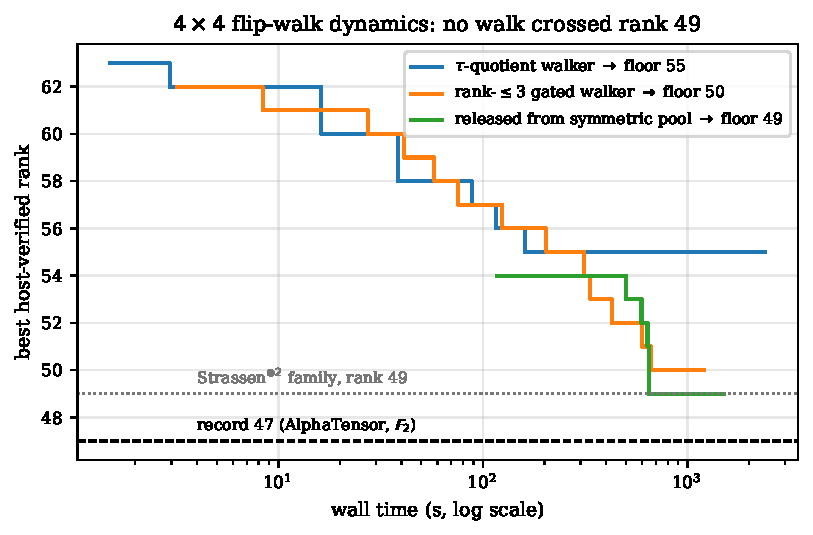
\includegraphics[width=0.78\textwidth]{figures/figure1_walker_floors.pdf}
\caption{Best host-verified rank against wall time for the three $4\times4$ walkers whose progress logs
recorded rank changes. The $\tau$-quotient walker descends fastest but stops at 55; the walk released
from the symmetric pool re-enters the rank-49 family; the factor-rank-gated walk stops at 50. No dynamic
crossed 49.}
\label{fig:walkers}
\end{figure}

\begin{figure}[htbp]
\centering
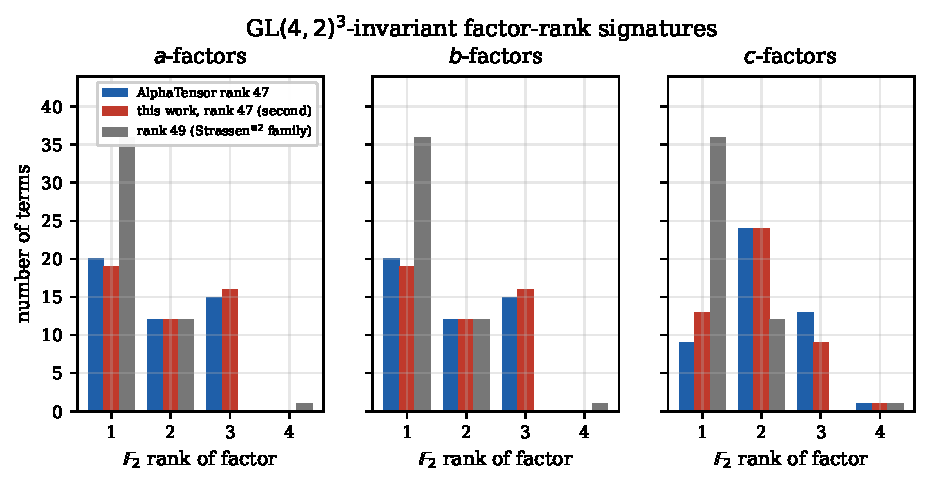
\includegraphics[width=0.95\textwidth]{figures/figure2_signatures.pdf}
\caption{$\GL(4,2)^3$-invariant factor-rank signatures. The two rank-47 schemes differ on every axis, which
proves they are inequivalent under all changes of basis and slot symmetries (Section~\ref{sec:second47}).
Both are rich in rank-3 factors, which the rank-49 Strassen$^{\otimes2}$ family cannot have in any basis
(Section~\ref{sec:obstructions}).}
\label{fig:signatures}
\end{figure}

\begin{figure}[htbp]
\centering
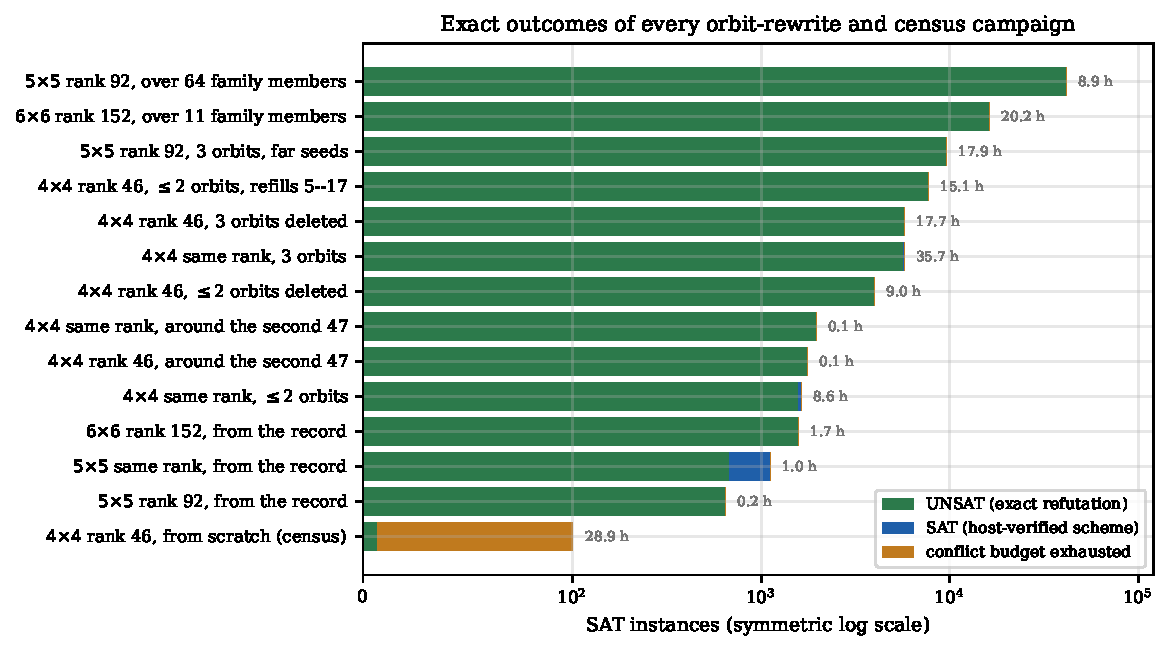
\includegraphics[width=0.92\textwidth]{figures/figure3_campaign_outcomes.pdf}
\caption{Outcomes of every exact campaign, on a symmetric log scale. Green is UNSAT (an exact
refutation), blue is a host-verified scheme, ochre is a conflict budget exhausted. Only the from-scratch
census leaves a substantial undecided remainder; every rewrite campaign terminated. Labels give solver
hours.}
\label{fig:campaigns}
\end{figure}

\begin{figure}[htbp]
\centering
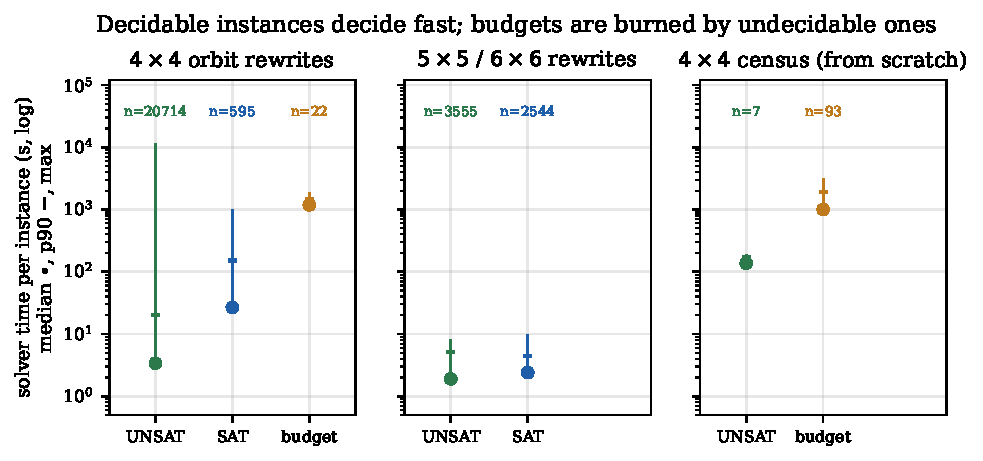
\includegraphics[width=0.95\textwidth]{figures/figure4_solve_times.pdf}
\caption{Solver time per instance. In every campaign the decidable instances decide within seconds to a
few minutes, while budget exhaustions sit two to three orders of magnitude to the right. This is what
justifies the policy of short sweep budgets followed by targeted re-runs.}
\label{fig:times}
\end{figure}

\begin{figure}[htbp]
\centering
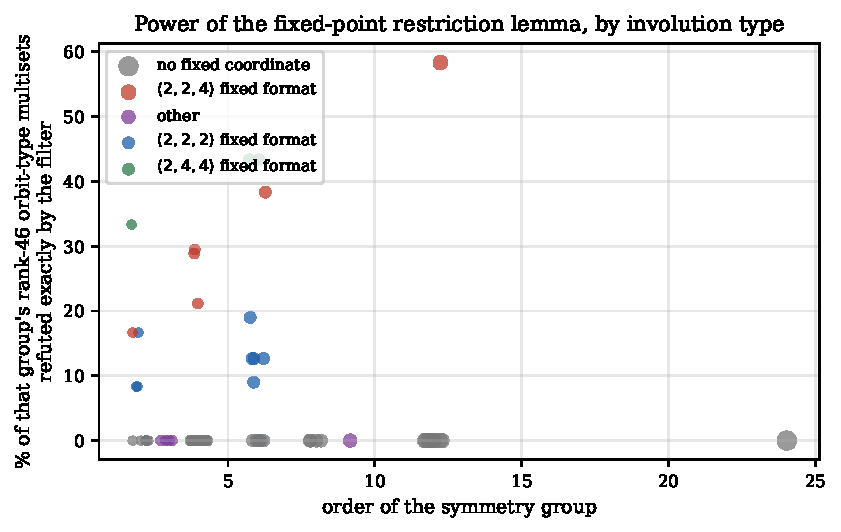
\includegraphics[width=0.78\textwidth]{figures/figure5_filter_power.pdf}
\caption{Fraction of each symmetry class's rank-46 orbit-type multisets refuted exactly by the
fixed-point filter, against group order, coloured by the fixed format of the class's involution.
Elimination is zero where the lemma has nothing to project onto and rises to 58\,\% for the order-12
class with a $\tw224$ fixed format. Marker area scales with group order.}
\label{fig:filter}
\end{figure}

\begin{figure}[htbp]
\centering
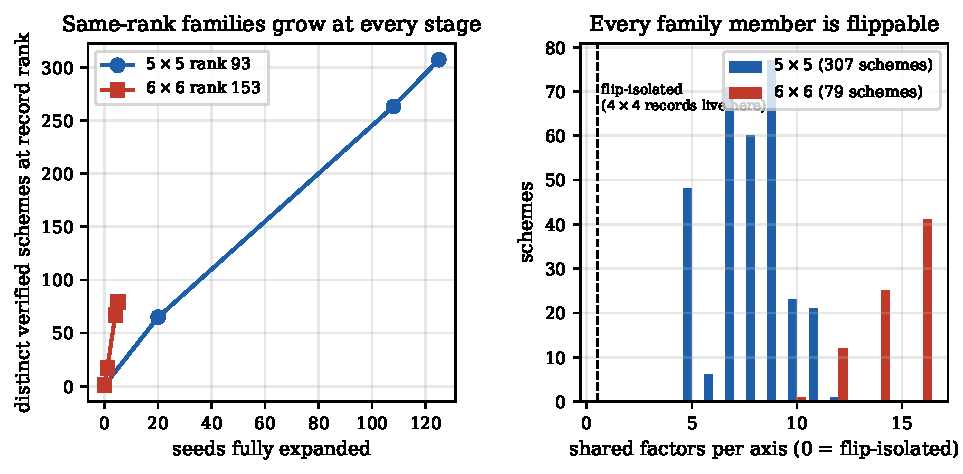
\includegraphics[width=0.95\textwidth]{figures/figure6_families.pdf}
\caption{Left: the same-rank families grow with every seed whose two-orbit neighbourhood is fully
enumerated, and neither is known to be finite. Right: shared factors per axis across the families; every
member is flippable, whereas both $4\times4$ rank-47 schemes sit at zero.}
\label{fig:families}
\end{figure}

\begin{figure}[htbp]
\centering
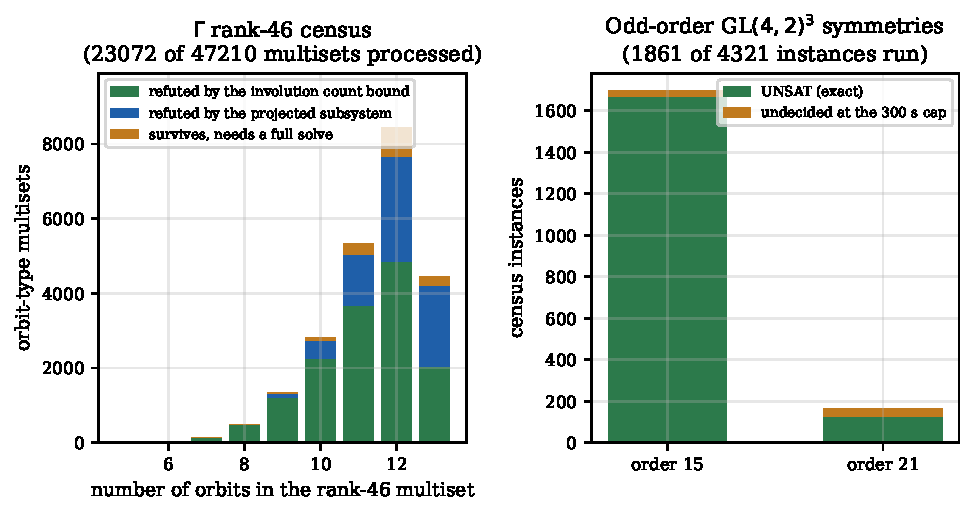
\includegraphics[width=0.95\textwidth]{figures/figure7_census.pdf}
\caption{Left: the $\Gamma$-invariant rank-46 census, by number of orbits in the multiset; nearly all
multisets are refuted by the count bound or the projected subsystem before any full solve is attempted.
Right: the odd-order general-linear census, complete for orders 15 and 21.}
\label{fig:census}
\end{figure}

\clearpage

\section{Discussion}

Three independent lines of evidence converge at $4\times4$. Every local dynamic falls into one
$\GL$-equivalence family at rank 49 and cannot leave it locally. Both known rank-47 schemes are
flip-isolated, so the flip-graph method cannot act on them or on anything equivalent to them. And both
are locally rigid under their own symmetry group, with no rank-46 neighbour within the tested radius. A
rank-46 scheme for $4\times4$ over $\FF$, if one exists, is therefore not a local modification of either
known 47 under $\Gamma$, not reachable by flip walks from the Strassen$^{\otimes2}$ family, and would
have to be found under a different symmetry group or by a construction that is non-local in the term set.

The contrast with $5\times5$ and $6\times6$ is sharp and, we think, the most useful observation in this
paper. There the records are flippable, non-rigid and cheap to rewrite, and they sit in families of
hundreds of same-rank schemes that our machinery enumerates in hours. Yet nothing descends: not exact
three-orbit rewrites where we ran them, and not $8.4\times10^{11}$ flip steps from 295 distinct seeds.
Same-rank families appear to be the norm and descent the exception, which suggests that the useful
question is less ``where is the next scheme'' than ``what distinguishes the rare rank-decreasing rewrite
from the overwhelming majority of rank-preserving ones.''

The fixed-point corollary points at one constructive answer that we did not have time to build. It says
that any involution-symmetric scheme carries a scheme for a smaller format among its fixed terms; a
rank-46 scheme with $f$ fixed terms has $(46-f)/2$ paired terms, so enumerating the small-format part
first and solving the paired complement second decomposes one hard instance into many small ones. Our
single calibration of this idea was negative --- pinning the 47's 9-term fixed core and asking for the 19
free pairs was undecided at $5\times10^6$ conflicts --- which suggests a single involution is too weak and
that the construction needs a Klein four-group or larger, gluing three sub-cores at once.

\section{Limitations and Future Work}
\label{sec:future}

\begin{itemize}
\item \textbf{Finish the censuses.} The $\Gamma$ rank-46 census is halfway through its filter stage, with
1{,}425 survivors already enumerated and the 9- to 11-orbit tier (403 instances) the natural next batch,
at a calibrated cost of hours each. The general-linear census has 2{,}460 instances left, at orders 35
and 105 where the instances are smallest.
\item \textbf{Twisted embeddings and Klein-four families.} The permutation census covered diagonal
embeddings of $S_4$-subgroups; the twisted embeddings --- of which $\Gamma$ itself is one --- are exactly
the region where the only known sub-49 objects live, and are not yet enumerated.
\item \textbf{Canonical enumeration of rank-8 $\tw222$ term sets.} The ladder construction needs the
class list, not the raw sets; a raw SAT enumeration passed 186{,}200 sets before we stopped it, so a
canonical-form enumeration is required.
\item \textbf{Mixed symmetries.} Slot rotation or transposition composed with a general-linear element is
untouched, and it is the natural generalisation of the symmetry the $5\times5$ and $6\times6$ records
actually have.
\item \textbf{Independent proof checking.} DRAT proofs were emitted for a sample of theorem-grade
refutations through Glucose 4.2 at no extra cost over the CaDiCaL solve, but no proof checker was
installed. Running a checker over the Theorem~\ref{thm:t1}--\ref{thm:t47b} instances would put those
theorems on machine-checked footing.
\item \textbf{Solver caveats.} Two PySAT bindings were excluded on evidence during this work: Kissat
4.0.4 returned a wrong answer on a five-clause formula and then crashed, and CaDiCaL 3.0.0 crashed
silently. All results here use CaDiCaL 1.9.5.
\end{itemize}

\section{Conclusion}

An exact, symmetry-stratified search on one laptop did not beat AlphaTensor's rank-47 scheme for
$4\times4$ over $\FF$, and produced a second, inequivalent rank-47 scheme instead; proved both to be
rigid and isolated within their symmetry class; introduced a fixed-point restriction lemma that refutes
symmetry classes at negligible cost and re-derives $\mathrm{rank}_{\FF}\tw222=7$; and turned the single
known $5\times5$ and $6\times6$ record schemes into families of 307 and 79 verified members that are not
known to be finite. Whether $\mathrm{rank}_{\FF}\tw444 \leq 46$ remains open. All code, all per-instance
logs and all verified schemes are archived with this paper.

\section*{Acknowledgments}

We thank the authors of CaDiCaL and PySAT, the maintainers of the Lille FMM database for publishing the
$5\times5$ and $6\times6$ schemes in reusable form, and the AlphaTensor authors for publishing their
factorizations. Computations performed on an NVIDIA GeForce RTX 5070 Laptop GPU and 12 CPU cores.

\section*{Code and Data Availability}

\begin{itemize}
\item Code, logs, verified schemes and both papers: this archive (see \texttt{README.md}).
\item Every headline number in this paper is regenerated from the raw result files by
\texttt{paper\_data.py}, every figure by \texttt{paper\_figures.py}, and the campaign's own
checklist by \texttt{reproduce.py} (21 checks, 0 mismatches), all under \texttt{experiments/}.
\end{itemize}

\bibliographystyle{plain}
\begin{thebibliography}{99}

\bibitem{Strassen1969}
V. Strassen, ``Gaussian elimination is not optimal,'' \emph{Numerische Mathematik}, 13:354--356, 1969.

\bibitem{Winograd1971}
S. Winograd, ``On multiplication of $2\times2$ matrices,'' \emph{Linear Algebra and its Applications},
4(4):381--388, 1971.

\bibitem{Laderman1976}
J. D. Laderman, ``A noncommutative algorithm for multiplying $3\times3$ matrices using 23
multiplications,'' \emph{Bulletin of the American Mathematical Society}, 82(1):126--128, 1976.

\bibitem{Brent1970}
R. P. Brent, ``Algorithms for matrix multiplication,'' Technical Report CS-157, Stanford University,
1970.

\bibitem{Fawzi2022}
A. Fawzi et al., ``Discovering faster matrix multiplication algorithms with reinforcement learning,''
\emph{Nature}, 610:47--53, 2022. \url{https://doi.org/10.1038/s41586-022-05172-4}; factorizations:
\url{https://github.com/google-deepmind/alphatensor}

\bibitem{Kauers2022}
M. Kauers, J. Moosbauer, ``Flip graphs for matrix multiplication,'' ISSAC 2023; arXiv:2212.01175.
\url{https://arxiv.org/abs/2212.01175}

\bibitem{Arai2024}
Y. Arai, Y. Ichikawa, K. Hukushima, ``Adaptive flip graph algorithm for matrix multiplication,'' ISSAC
2024; arXiv:2312.16960. \url{https://arxiv.org/abs/2312.16960}

\bibitem{Moosbauer2025}
J. Moosbauer, M. Poole, ``Flip graphs with symmetry and new matrix multiplication schemes,''
arXiv:2502.04514, 2025. \url{https://arxiv.org/abs/2502.04514}

\bibitem{fmmdb}
Fast Matrix Multiplication database, Universit\'e de Lille. \url{https://fmm.univ-lille.fr}

\bibitem{Blaser2003}
M. Bl\"aser, ``On the complexity of the multiplication of matrices of small formats,'' \emph{Journal of
Complexity}, 19(1):43--60, 2003.

\bibitem{cadical}
A. Biere et al., ``CaDiCaL, Kissat, Paracooba, Plingeling and Treengeling entering the SAT Competition,''
\emph{Proceedings of SAT Competition}, 2020.

\bibitem{pysat}
A. Ignatiev, A. Morgado, J. Marques-Silva, ``PySAT: A Python toolkit for prototyping with SAT oracles,''
\emph{SAT 2018}, LNCS 10929, pp. 428--437.

\end{thebibliography}

\end{document}
